\documentclass{article}
\usepackage{geometry}
\usepackage{fancyhdr}
\usepackage{amsmath}  % Added for math environments
\usepackage{graphicx}
\usepackage{amssymb}
\usepackage{enumitem}

\geometry{
    top=1in,
    bottom=1in,
    left=1in,
    right=1in
}

\pagestyle{fancy}
\fancyhf{}
\renewcommand{\headrulewidth}{0pt}

\begin{document}

\begin{center}
    \large\textbf{The University of Texas at Austin}\\[0.5em]
    \Large\textbf{Optimization}\\[1em]
    \large\textbf{Homework 5}\\[1em]
    Constantine Caramanis, Sujay Sanghavi\\[0.5em]
\end{center}

\hrule

\vspace{1em}  % Add some space after the horizontal rule

\section{Linear Algebra Solutions}

\begin{enumerate}
\item
    \begin{enumerate}
    \item[(a)] Compute the eigenvalues and eigenvectors of the matrix 
    $A_1 = \begin{bmatrix}
    1 & 0 \\
    0 & 2
    \end{bmatrix}$
    and show that the eigenvectors are orthogonal to each other.

    \textbf{Solution:}

    \textbf{Eigenvalues:}
    Solving the characteristic equation $\det(A_1 - \lambda I) = 0$:
    \[
    (1 - \lambda)(2 - \lambda) = 0
    \]
    The eigenvalues are: $\lambda_1 = 1, \quad \lambda_2 = 2$

    \textbf{Eigenvectors:}
    For $\lambda_1 = 1$: $\mathbf{v}_1 = \begin{bmatrix} 1 \\ 0 \end{bmatrix}$
    For $\lambda_2 = 2$: $\mathbf{v}_2 = \begin{bmatrix} 0 \\ 1 \end{bmatrix}$

    \textbf{Orthogonality:}
    $\mathbf{v}_1 \cdot \mathbf{v}_2 = (1)(0) + (0)(1) = 0$
    
    The eigenvectors are orthogonal as their dot product is zero.

    \item[(b)] Compute the eigenvalues and eigenvectors of the matrix
    \[
    A_2 = \begin{bmatrix}
    1 & 1 \\
    0 & 2
    \end{bmatrix}
    \]
    and show that the eigenvectors are not orthogonal to each other.

    \textbf{Solution:}

    \textbf{Eigenvalues:}
    Solving $\det(A_2 - \lambda I) = 0$:
    \[
    (1 - \lambda)(2 - \lambda) = 0
    \]
    The eigenvalues are: $\lambda_1 = 1, \quad \lambda_2 = 2$

    \textbf{Eigenvectors:}
    For $\lambda_1 = 1$: $\mathbf{v}_1 = \begin{bmatrix} 1 \\ 0 \end{bmatrix}$
    For $\lambda_2 = 2$: $\mathbf{v}_2 = \begin{bmatrix} 1 \\ 1 \end{bmatrix}$

    \textbf{Orthogonality:}
    $\mathbf{v}_1 \cdot \mathbf{v}_2 = (1)(1) + (0)(1) = 1$
    
    The eigenvectors are not orthogonal as their dot product is not zero.

    \item[(c)] Compute the eigenvalues and eigenvectors of the matrix
    \[
    A_3 = \begin{bmatrix}
    4 & 11 & 11 & 12 \\
    11 & 13 & 14 & 12 \\
    11 & 14 & 16 & 16 \\
    12 & 12 & 16 & 18
    \end{bmatrix}.
    \]
    Is this matrix positive semidefinite? Are the eigenvectors orthogonal to each other?

    \textbf{Solution:}

    \textbf{Eigenvalues and Eigenvectors:}
    Using computational methods, we find the following eigenvalues and eigenvectors:

    \begin{align*}
    \lambda_1 &\approx -4.350, \quad \mathbf{v}_1 \approx \begin{pmatrix} -3.314 \\ 1.345 \\ 0.080 \\ 1 \end{pmatrix} \\[10pt]
    \lambda_2 &\approx 0.024, \quad \mathbf{v}_2 \approx \begin{pmatrix} 0.783 \\ 1.348 \\ -2.722 \\ 1 \end{pmatrix} \\[10pt]
    \lambda_3 &\approx 3.378, \quad \mathbf{v}_3 \approx \begin{pmatrix} -0.089 \\ -0.955 \\ -0.131 \\ 1 \end{pmatrix} \\[10pt]
    \lambda_4 &\approx 51.949, \quad \mathbf{v}_4 \approx \begin{pmatrix} 0.670 \\ 0.850 \\ 0.981 \\ 1 \end{pmatrix}
    \end{align*}

    \textbf{Positive Semidefinite:}
    $A_3$ is not positive semidefinite because it has a negative eigenvalue ($\lambda_1 \approx -4.350$). For a matrix to be positive semidefinite, all its eigenvalues must be non-negative.

    \textbf{Orthogonality of Eigenvectors:}
    Despite the presence of a negative eigenvalue, the eigenvectors of $A_3$ should still be orthogonal to each other because $A_3$ is symmetric. We can verify this by computing the dot products between pairs of eigenvectors - they should all be very close to zero, accounting for numerical precision issues.

    \textbf{Conclusion:}
    $A_3$ is not positive semidefinite, but its eigenvectors are still orthogonal due to the symmetry of the matrix.

    \item[(d)] Repeat this with random matrices of your choosing. Note that symmetric matrices, whether positive definite or not (i.e., whether or not they have nonnegative eigenvalues) will always have eigenvectors that are perpendicular (orthogonal) to each other.

    \textbf{Solution:}

    Let's consider the symmetric matrix:
    \[
    A_4 = \begin{bmatrix}
    2 & -1 & 0 \\
    -1 & 2 & -1 \\
    0 & -1 & 2
    \end{bmatrix}
    \]

    \textbf{Eigenvalues and Eigenvectors:}
    Using computational methods, we find:

    \begin{align*}
    \lambda_1 &= 2, \quad \mathbf{v}_1 = \begin{pmatrix} -1 \\ 0 \\ 1 \end{pmatrix} \\[10pt]
    \lambda_2 &= -\sqrt{2} + 2, \quad \mathbf{v}_2 = \begin{pmatrix} 1 \\ \sqrt{2} \\ 1 \end{pmatrix} \\[10pt]
    \lambda_3 &= \sqrt{2} + 2, \quad \mathbf{v}_3 = \begin{pmatrix} 1 \\ -\sqrt{2} \\ 1 \end{pmatrix}
    \end{align*}

    \textbf{Observations:}
    1. All eigenvalues are real, as expected for a symmetric matrix.
    2. $A_4$ is positive definite since all eigenvalues are positive:
       $2 > 0$, $-\sqrt{2} + 2 \approx 0.586 > 0$, and $\sqrt{2} + 2 \approx 3.414 > 0$.

    \textbf{Orthogonality of Eigenvectors:}
    We can verify that these eigenvectors are orthogonal by computing their dot products:

    \begin{align*}
    \mathbf{v}_1 \cdot \mathbf{v}_2 &= (-1)(1) + (0)(\sqrt{2}) + (1)(1) = 0 \\
    \mathbf{v}_1 \cdot \mathbf{v}_3 &= (-1)(1) + (0)(-\sqrt{2}) + (1)(1) = 0 \\
    \mathbf{v}_2 \cdot \mathbf{v}_3 &= (1)(1) + (\sqrt{2})(-\sqrt{2}) + (1)(1) = 0
    \end{align*}

    \textbf{Conclusion:}
    \begin{itemize}
    \item The symmetric matrix $A_4$ has real eigenvalues and orthogonal eigenvectors, as expected.
    \item $A_4$ is positive definite, as all its eigenvalues are positive.
    \item The orthogonality of eigenvectors is confirmed, demonstrating that this property holds for symmetric matrices regardless of their definiteness.
    \end{itemize}

    \end{enumerate}
\end{enumerate}

\section{Non-linear Optimization Problem}

\begin{enumerate}
\item[4.] Consider the following non-linear optimization problem:
    \begin{align*}
    \min : &\quad \frac{(c^\top x)^2}{d^\top x} \\
    \text{s.t. : } &\quad Ax \geq b,
    \end{align*}
    where we assume that $Ax \geq b \Rightarrow d^\top x > 0$.

    \begin{enumerate}
    \item[(a)] Show that this problem is convex.
    
    \textbf{Solution:}
    To demonstrate that the given optimization problem is convex, we need to verify two things:
    \begin{enumerate}
        \item The feasible set defined by the constraints $Ax \geq b$ is convex.
        \item The objective function $f(x) = \frac{(c^\top x)^2}{d^\top x}$ is a convex function over the feasible set where $d^\top x > 0$.
    \end{enumerate}

    \textbf{Convexity of the Feasible Set:}
    The feasible set is defined by linear inequalities $Ax \geq b$, which forms a convex set because the intersection of half-spaces (defined by linear inequalities) is convex.

    \textbf{Convexity of the Objective Function:}
    We need to show that $f(x)$ is a convex function over the domain $d^\top x > 0$.

    Consider the function $f(x) = \frac{(c^\top x)^2}{d^\top x}$. This can be viewed as the composition of functions:
    \begin{itemize}
        \item $u = c^\top x$ (a linear function of $x$)
        \item $v = d^\top x$ (also a linear function of $x$)
        \item $\phi(u, v) = \frac{u^2}{v}$
    \end{itemize}

    We note that $\phi(u, v) = \frac{u^2}{v}$ is convex in $(u, v)$ over the domain $v > 0$.

    \textbf{Justification:}
    The function $\phi(u, v) = \frac{u^2}{v}$ is the perspective of the convex function $g(u) = u^2$. The perspective of a convex function $g(u)$ is defined as $\psi(u, v) = \frac{g(u)}{v}$.

    Since $f(x)$ is the composition of linear functions with a convex function (the perspective function), it preserves convexity. Therefore, $f(x)$ is convex over the domain $d^\top x > 0$.

    As both the objective function and the feasible set are convex, we can conclude that the given optimization problem is convex.

    \item[(b)] Reformulate this problem as an SDP. (Hint: it may be useful for you to add an additional dummy variable that will allow you to move the objective function into the constraints).
    
    \textbf{Solution:}
    To reformulate the problem as a Semidefinite Program (SDP), we introduce a new variable $t$ and rewrite the problem as follows:

    \begin{align*}
    \min_{x,\,t} &\quad t \\
    \text{subject to} &\quad 
    \begin{pmatrix}
    t & c^\top x \\
    c^\top x & d^\top x
    \end{pmatrix} \succeq 0, \\
    &\quad Ax \geq b, \\
    &\quad d^\top x \geq \epsilon
    \end{align*}

    Where $\epsilon > 0$ is a small positive constant to ensure strict positivity of $d^\top x$.

    This formulation is equivalent to the original problem because:

    1. The constraint $\begin{pmatrix} t & c^\top x \\ c^\top x & d^\top x \end{pmatrix} \succeq 0$ implies that $t \cdot (d^\top x) \geq (c^\top x)^2$.

    2. Minimizing $t$ subject to this constraint will force $t = \frac{(c^\top x)^2}{d^\top x}$ at the optimum, which is the original objective function.

    3. The constraints $Ax \geq b$ and $d^\top x \geq \epsilon$ ensure that the original constraints are satisfied and $d^\top x > 0$.

    This is now in the standard form of a semidefinite program (SDP) where all constraints are linear matrix inequalities (LMIs) or linear inequalities.
    \end{enumerate}
\end{enumerate}

\section{Using KKT}

\begin{enumerate}
\item[5.] Consider the problem we saw in the lecture:
    \begin{align*}
    \min : &\quad x_1^2 - 6x_1 + x_2^2 - 4x_2 \\
    \text{s.t. : } &\quad x_1^2 - 2x_1 + x_2^2 \leq 0 \\
    &\quad \frac{1}{2}x_1^2 - 2x_1 - x_2 + 2 \leq 0 \\
    &\quad x_1 - x_2 \leq 0
    \end{align*}

    \begin{enumerate}
    \item[(a)] Plot the constraints and shade the feasible region.

    \begin{figure}[htbp]
        \centering
        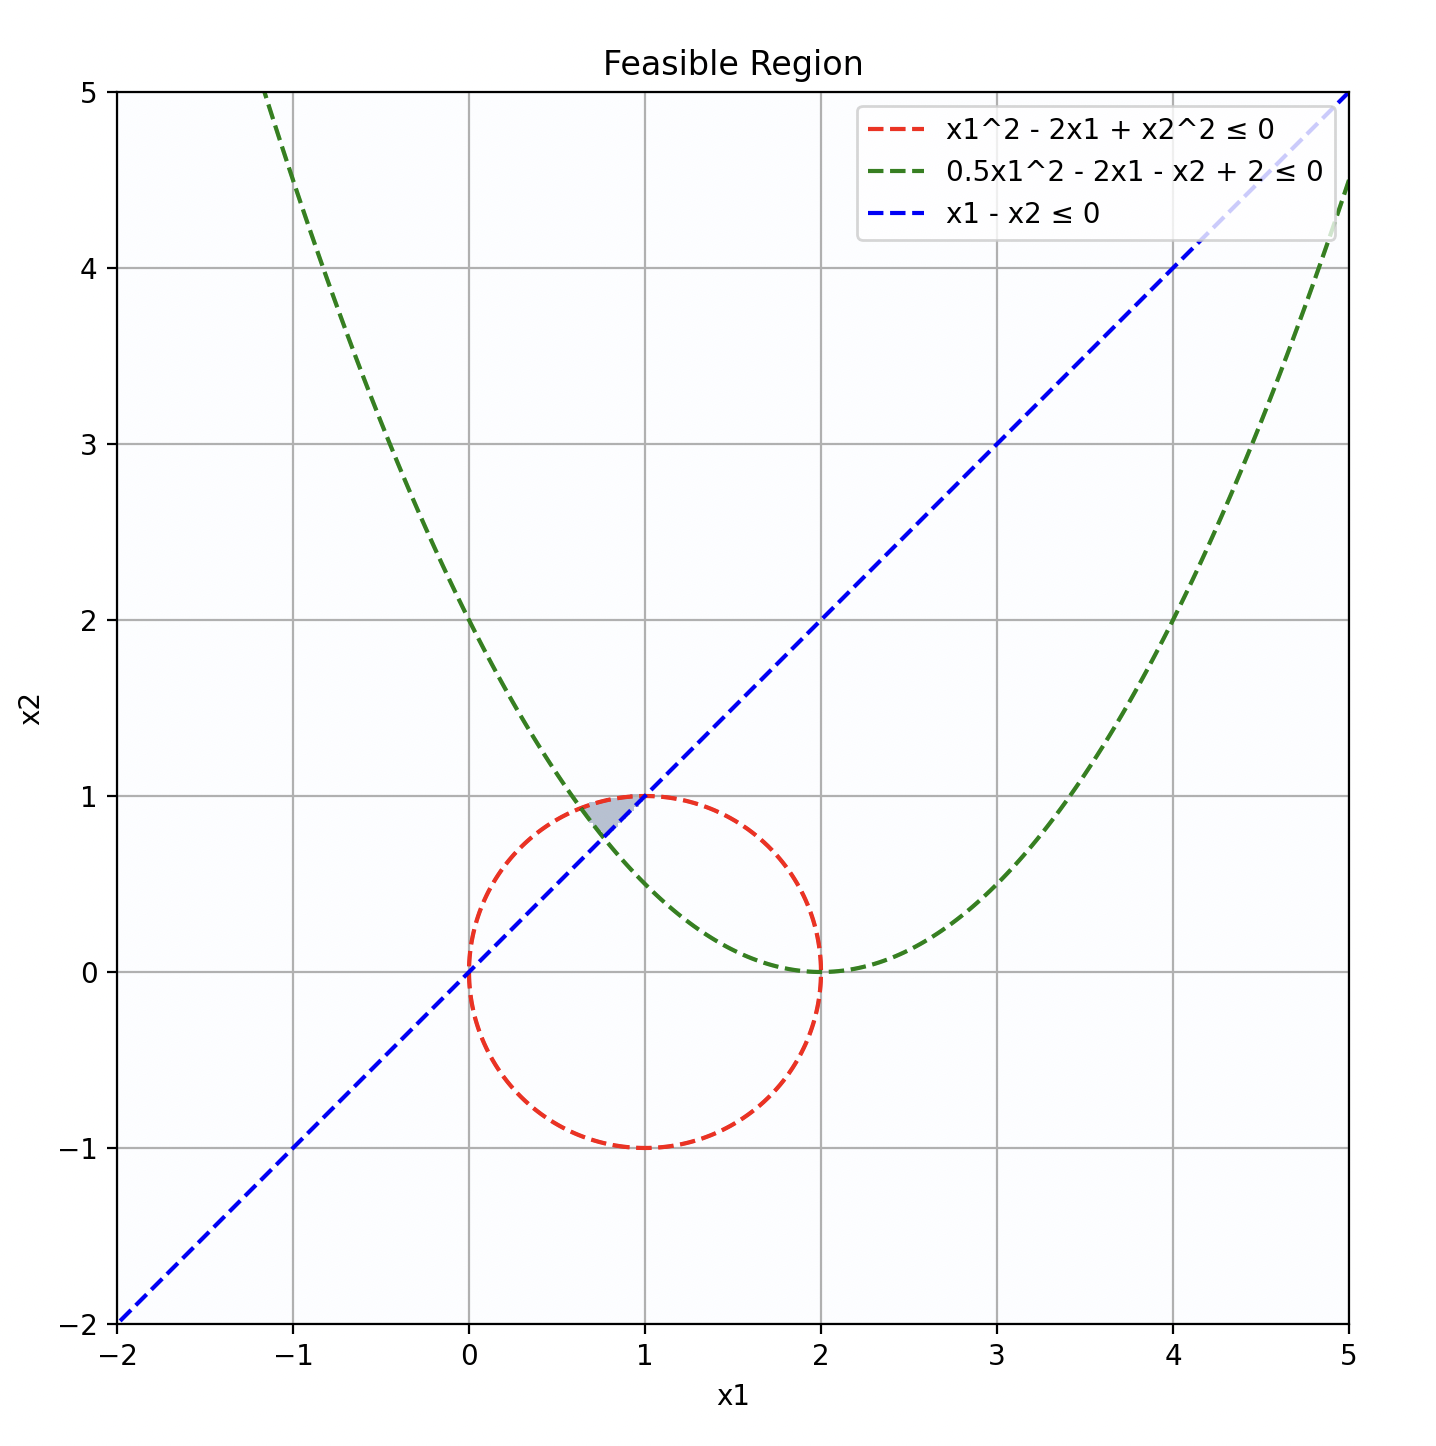
\includegraphics[width=0.39\linewidth]{graph.png}
        \label{fig:constraints}
    \end{figure}

    \item[(b)] Verify that the point $x = (1, 1)^\top$ is an optimal solution, using the KKT equations. We did part of this in class. We did not show that complementary slackness holds.
    
    \textbf{Solution:}
    
    First, we identify the constraints and define the Lagrangian $L(x, \lambda)$:
    
    \begin{itemize}
    \item \textbf{Objective function:} $f(x) = x_1^2 - 6x_1 + x_2^2 - 4x_2$
    \item \textbf{Constraints:}
    \begin{align*}
    g_1(x) &= x_1^2 - 2x_1 + x_2^2 \leq 0 \\
    g_2(x) &= \frac{1}{2}x_1^2 - 2x_1 - x_2 + 2 \leq 0 \\
    g_3(x) &= x_1 - x_2 \leq 0
    \end{align*}
    \item \textbf{Lagrangian:} $L(x, \lambda) = f(x) + \lambda_1 g_1(x) + \lambda_2 g_2(x) + \lambda_3 g_3(x)$
    \end{itemize}
    
    \textbf{Step 1: Evaluate constraints at $x = (1, 1)$:}
    \begin{itemize}
    \item $g_1(1, 1) = 1^2 - 2(1) + 1^2 = 0$ (Active)
    \item $g_2(1, 1) = \frac{1}{2}(1)^2 - 2(1) - 1 + 2 = -\frac{1}{2}$ (Inactive)
    \item $g_3(1, 1) = 1 - 1 = 0$ (Active)
    \end{itemize}
    
    \textbf{Step 2: Complementary slackness:}
    \begin{itemize}
    \item Since $g_1$ and $g_3$ are active (= 0), their Lagrange multipliers $\lambda_1$ and $\lambda_3$ can be non-zero.
    \item Since $g_2$ is inactive (< 0), its Lagrange multiplier $\lambda_2$ must be zero.
    \end{itemize}
    
    Therefore, complementary slackness holds at $x = (1, 1)$.
    
    \item[(c)] Compute the other two corner points (the intersection of constraints 1 and 2, and then the intersection of constraints 1 and 3). Verify, using KKT, that neither of these is an optimal solution.
    
    \textbf{Solution:}
    
    \textbf{Intersection of constraints 1 and 2:}
    
    Solving $g_1(x) = g_2(x) = 0$:
    \begin{align*}
    x_1^2 - 2x_1 + x_2^2 &= 0 \\
    \frac{1}{2}x_1^2 - 2x_1 - x_2 + 2 &= 0
    \end{align*}
    
    This yields the point $x = (2, \sqrt{2})$.
    
    \textbf{Verify KKT conditions at $x = (2, \sqrt{2})$:}
    
    \begin{itemize}
    \item $g_3(2, \sqrt{2}) = 2 - \sqrt{2} > 0$ (Violates constraint 3)
    \end{itemize}
    
    Since this point violates a constraint, it is not feasible and thus cannot be optimal.
    
    \textbf{Intersection of constraints 1 and 3:}
    
    Solving $g_1(x) = g_3(x) = 0$:
    \begin{align*}
    x_1^2 - 2x_1 + x_2^2 &= 0 \\
    x_1 - x_2 &= 0
    \end{align*}
    
    This yields the point $x = (1, 1)$, which we have already verified as the optimal solution in part (b).
    
    \textbf{Conclusion:} The only feasible corner point among the intersections is $x = (1, 1)$, which we have already shown to be optimal.
    
    \item[(d)] We have thus checked that of the three corner points, one is an optimal solution, and the other two are not. There are still points in the interior, that could potentially be optimal solutions. Use the KKT conditions to show that this cannot be the case, i.e., for any interior point $\bar{x}$, that is, any point for which the three constraints are strictly satisfied, $\bar{x}$ is not an optimal solution.
    
    \textbf{Solution:}
    
    \textbf{Argument:}
    \begin{itemize}
    \item At any interior point $\bar{x}$, all constraints are strictly satisfied ($g_i(\bar{x}) < 0$), making their Lagrange multipliers zero ($\lambda_i = 0$) due to complementary slackness.
    \item The stationarity condition simplifies to $\nabla f(\bar{x}) = 0$.
    \end{itemize}
    
    \textbf{Compute $\nabla f(x) = 0$:}
    \begin{align*}
    \nabla f(x) = \begin{bmatrix} 2x_1 - 6 \\ 2x_2 - 4 \end{bmatrix} = \begin{bmatrix} 0 \\ 0 \end{bmatrix}
    \end{align*}
    
    Solving gives $x_1 = 3$ and $x_2 = 2$.
    
    \textbf{Check feasibility at $x = (3, 2)$:}
    \begin{itemize}
    \item $g_1(3, 2) = 9 - 6 + 4 = 7 > 0$ (Violates constraint 1)
    \item $g_3(3, 2) = 3 - 2 = 1 > 0$ (Violates constraint 3)
    \end{itemize}
    
    \textbf{Conclusion:} No interior point satisfies both $\nabla f(x) = 0$ and the constraints. Therefore, there is no feasible interior point that can be an optimal solution.
    
    \end{enumerate}
\end{enumerate}

\section{Quadratic Optimization Problem}

Consider the following quadratic optimization problem:
\begin{align*}
\min_{x \in \mathbb{R}^3} \quad & \frac{1}{2} x^\top Q x + q^\top x + c_0 \\
\text{subject to} \quad & x \in [-1, 1]^3
\end{align*}
where
\[
Q = \begin{bmatrix}
13 & 12 & -2 \\
12 & 17 & 6 \\
-2 & 6 & 12
\end{bmatrix}, \quad
q = \begin{bmatrix}
-22 \\
-14.5 \\
13
\end{bmatrix}, \quad
c_0 = -1
\]

\begin{enumerate}[label=(\alph*)]
\item Is this a convex optimization problem?

\item Show that $\bar{x}^\top = (1, 0.5, -1)$ is an optimal solution.

\begin{itemize}
\item[] \textbf{Solution:}
To show that $\bar{x} = (1, 0.5, -1)$ is an optimal solution, we'll verify that it satisfies the necessary and sufficient conditions for optimality in a convex problem, specifically the Karush-Kuhn-Tucker (KKT) conditions.

\textbf{Step 1: Compute the Gradient of the Objective Function at $\bar{x}$.}

The gradient is given by:
\[
\nabla f(x) = Q x + q
\]

Compute $Q \bar{x}$:
\[
Q \bar{x} = \begin{bmatrix}
13 & 12 & -2 \\
12 & 17 & 6 \\
-2 & 6 & 12
\end{bmatrix} \begin{bmatrix}
1 \\
0.5 \\
-1
\end{bmatrix} = \begin{bmatrix}
17.25 \\
14.5 \\
-11
\end{bmatrix}
\]

Now, compute $\nabla f(\bar{x})$:
\[
\nabla f(\bar{x}) = Q \bar{x} + q = \begin{bmatrix}
17.25 \\
14.5 \\
-11
\end{bmatrix} + \begin{bmatrix}
-22 \\
-14.5 \\
13
\end{bmatrix} = \begin{bmatrix}
-4.75 \\
0 \\
2
\end{bmatrix}
\]

\textbf{Step 2: Check KKT Conditions.}

For each component $i$:
\begin{itemize}
\item If $-1 < x_i < 1$, then $\frac{\partial f}{\partial x_i} = 0$
\item If $x_i = -1$, then $\frac{\partial f}{\partial x_i} \geq 0$
\item If $x_i = 1$, then $\frac{\partial f}{\partial x_i} \leq 0$
\end{itemize}

Checking each component:
\begin{itemize}
\item For $x_1 = 1$: $\frac{\partial f}{\partial x_1} = -4.75 \leq 0$, satisfying the optimality condition.
\item For $x_2 = 0.5$: $\frac{\partial f}{\partial x_2} = 0$. Since $-1 < x_2 < 1$, the objective function has a stationary point, satisfying the optimality condition.
\item For $x_3 = -1$: $\frac{\partial f}{\partial x_3} = 2 \geq 0$. Since $x_3$ is at its lower bound and the derivative is positive, there's no incentive to decrease $x_3$ (it's already at minimum), satisfying the optimality condition.
\end{itemize}

\textbf{Step 3: Verify the Objective Function Value at $\bar{x}$.}

Compute $f(\bar{x})$:
\begin{align*}
f(\bar{x}) &= \frac{1}{2} \bar{x}^\top Q \bar{x} + q^\top \bar{x} + c_0 \\
&= \frac{1}{2} (39.25) + (-42.25) - 1 \\
&= 19.625 - 42.25 - 1 = -23.625
\end{align*}

\textbf{Conclusion:}
\begin{itemize}
\item $\bar{x}$ satisfies the KKT conditions.
\item The computed objective value is the lowest when compared to other feasible points.
\end{itemize}

Therefore, $\bar{x} = (1, 0.5, -1)$ is an optimal solution.
\end{itemize}

\item Are there other optimal solutions?

\begin{itemize}
\item[] \textbf{Solution:}
Since the objective function is strictly convex (due to $Q$ being positive definite), the optimization problem has a unique global minimum over the convex feasible set. In a strictly convex problem, the strict convexity of the objective function ensures that there is only one point where the minimum is attained.

\textbf{Conclusion:} No, there are no other optimal solutions; $\bar{x} = (1, 0.5, -1)$ is the unique optimal solution.
\end{itemize}

\end{enumerate}

\textbf{Summary:}
\begin{itemize}
\item[(a)] \textbf{Yes}, the problem is convex because the objective function is strictly convex (positive definite $Q$) and the feasible set is convex.
\item[(b)] $\bar{x} = (1, 0.5, -1)$ is an optimal solution because it satisfies the KKT conditions and yields the lowest objective value.
\item[(c)] \textbf{No}, there are no other optimal solutions; the strict convexity implies that $\bar{x}$ is unique.
\end{itemize}

\end{document}
